\documentclass[11pt, a4paper]{article}

\usepackage{amsmath}
\usepackage{amssymb}
\usepackage{array}
\usepackage{longtable}
\usepackage{multirow}
\usepackage{listings}
\usepackage{xcolor}
\usepackage{siunitx}
\usepackage{seqsplit}
\usepackage{kotex}
\usepackage{booktabs}
\usepackage{caption}
\usepackage{tabularx}
\usepackage{makecell}
\usepackage{float}
\usepackage{graphicx}
\usepackage{titlesec}

\titlespacing*{\section}{0pt}{1.2ex plus 0.4ex minus 0.2ex}{0.6ex plus 0.1ex}
\titlespacing*{\subsection}{0pt}{1.0ex plus 0.3ex minus 0.1ex}{0.4ex plus 0.1ex}
\titlespacing*{\subsubsection}{0pt}{0.8ex plus 0.2ex minus 0.1ex}{0.2ex plus 0.1ex}
\titlespacing*{\paragraph}{0pt}{0.6ex plus 0.1ex minus 0.1ex}{0.4em}

\usepackage{titling}
\setlength{\droptitle}{-4em}
\posttitle{\end{center}\vspace{-1.5em}}
\preauthor{\begin{center}}
\postauthor{\end{center}\vspace{-6em}}

\usepackage{fontspec}
\setmainfont{Noto Serif CJK KR}

\usepackage{geometry}
\geometry{margin=0.5in}

\usepackage{hyperref}
\hypersetup{
    colorlinks=true,
    linkcolor=blue,
    urlcolor=blue,
    citecolor=blue
}

\setlength{\parskip}{0.3em}
\setlength{\parindent}{1em}

\title{MIMIC 기반 기존 연구 리뷰 및 재현 보고서}
\author{2024404060 강민혁}
\date{}

\begin{document}

\maketitle

\section{서론}
본 보고서는 \textbf{``A New Evaluation Model for Traumatic Severe Pneumothorax Based on Interpretable Machine Learning''}~\cite{li2024} 논문을 재현하고 분석한다. 이 논문은 MIMIC-IV 데이터 기반으로 외상성 중증 기흉을 신속하게 평가하는 해석 가능한 머신러닝 모델을 제안하였다. 외상성 기흉은 신속한 진단이 생존율과 직결되는 응급 질환이므로, 영상 검사가 어려운 환경에서도 활용 가능한 예측 모델의 임상적 필요성이 높다. 기흉 병력이 있는 작성자는 임상 데이터만으로 질환을 예측할 수 있다는 점에 흥미를 느껴 해당 주제를 선정하였다.

\section{기존 논문 리뷰}
해당 연구는 MIMIC-IV를 활용하여 외상성 중증 기흉을 진단하는 해석 가능한 머신러닝 모델을 제안하였다. 활력 징후와 혈액 가스 분석에서 추출한 12가지 임상 변수(pH, Hemoglobin, PaO$_2$, Lactate 등)로 기흉 중증도를 조기 판별하는 모델을 구축하였다. 코호트는 실험군(외상성 중증 기흉 환자 174명)과 대조군(비외상성 비기흉 환자 3,697명, 1:5 다운샘플링 적용)으로 구성하였다.

Figure~\ref{fig:original_results}와 같이 4가지 기계학습 알고리즘 중 XGBoost가 AUROC 0.979, 정확도 0.947, 재현율 0.730으로 가장 우수한 성능을 보였다. SHAP 분석 결과, pH, Hemoglobin, PaO$_2$가 주요 예측 인자로 확인되었다.

\begin{figure}[htbp]
  \centering
  \includegraphics[width=0.75\textwidth]{figures/original_results.png}
  \caption{Original Research Performance Evaluation and SHAP Analysis Results}
  \label{fig:original_results}
\end{figure}

\section{재현 방법}
\subsection{코호트 구성}
원 논문의 선정 기준을 준수하여 코호트를 재구성하였으나 최종 규모에서 차이가 발생하였다. 원 논문에서는 실험군 174명, 대조군 3,697명을 추출하였으나, 본 연구에서는 초기 추출 시 실험군 195명, 대조군 10,174명을 확보한 후, ICU 입실 요건 및 결측률 기준 적용을 거쳐 최종적으로 실험군 119명, 대조군 544명을 분석에 포함하였다. 실험군은 ICD-10 진단코드, CheXpert/NegBio 라벨, CXR 리포트 텍스트 마이닝을 통해 선별하였으며, 원 논문의 영상 측정 기반 분류와 달리 텍스트 기반 추론에 의존하여 규모 차이가 발생하였다.

\subsection{데이터 전처리 및 모델링}
원 논문의 12개 변수에 FiO$_2$와 MAP를 추가하여 14개 변수를 수집하고, 결측률 기준(대조군 50\%, 실험군 85\%)을 적용하였다. 결측치는 MICE를 활용하여 5회 반복 대체 후 평균값을 사용하였다. 베이스라인 모델은 XGBoost로 그리드 서치를 통해 하이퍼파라미터를 탐색하였으며, 5-Fold 교차 검증을 통해 모델 성능을 평가하였다(상세 내용은 Appendix 참조).

\subsection{제안 모델}
베이스라인의 낮은 재현율 문제를 해결하기 위해 민감도 최적화 파이프라인을 설계하였다. (1) 클래스 불균형 해소를 위해 음성/양성 비율 기반 가중치에 2배를 추가 적용, (2) Optuna~\cite{akiba2019optuna}를 사용한 베이지안 최적화로 AUROC와 재현율을 결합한 목적 함수(Score = AUROC + 0.5 $\times$ Recall) 최적화, (3) 최소 민감도(Recall $\ge$ 0.45)와 최소 정확도(Accuracy $\ge$ 0.85) 제약을 만족하는 임계값 최적화를 수행하였다. Table~\ref{tab:hyperparameters_proposed}는 베이지안 최적화를 통해 도출된 최적 하이퍼파라미터이다.

\begin{table}[htbp]
  \centering
  \footnotesize
  \caption{Proposed Model XGBoost Hyperparameters via Bayesian Optimization}
  \label{tab:hyperparameters_proposed}
  \renewcommand{\arraystretch}{0.6}
  \setlength{\tabcolsep}{4pt}
  \begin{tabular}{l c l}
    \toprule
    \textbf{Hyperparameter} & \textbf{Symbol} & \textbf{Optimal Value} \\
    \midrule
    Number of Estimators & $M$ & 327 \\
    Max Depth & $d_{\max}$ & 10 \\
    Learning Rate & $\eta$ & 0.0117 \\
    Subsample Ratio & $r_{\text{sub}}$ & 0.959 \\
    Column Subsample Ratio & $r_{\text{col}}$ & 0.627 \\
    Min Child Weight & $w_{\min}$ & 2 \\
    Min Split Loss & $\gamma$ & 0.0096 \\
    L1 Regularization & $\alpha_{\text{reg}}$ & 0.0029 \\
    L2 Regularization & $\lambda_{\text{reg}}$ & $3.22 \times 10^{-8}$ \\
    \bottomrule
  \end{tabular}
\end{table}

\subsection{실행 환경}
본 과제는 Linux 환경(AMD Ryzen 9 5900X, 64GB RAM, NVIDIA RTX 3080)에서 수행되었으며, Python 3.12, XGBoost 2.0, Optuna 3.3 등을 사용하였다.

\section{실험 결과}
\subsection{성능 비교}
Table~\ref{tab:performance}는 원 논문, 베이스라인, 제안 모델의 성능을 비교한 결과이다.

\begin{table}[H]
\centering
\caption{Model Performance Comparison}
\label{tab:performance}
\footnotesize
\renewcommand{\arraystretch}{0.6}
\setlength{\tabcolsep}{3pt}
\resizebox{\textwidth}{!}{
  \begin{tabular}{llcccccc}
  \toprule
  Model & Accuracy & F1 & Precision & Recall & AUROC & AUPRC \\
  \midrule
  Original XGBoost & 0.947 & 0.822 & 0.941 & 0.730 & 0.979 & 0.926 \\
  Baseline (Repro.) & 0.885±0.016 & 0.557±0.076 & 0.779±0.083 & 0.442±0.082 & 0.910±0.038 & 0.764±0.066 \\
  Proposed Model & 0.883±0.034 & 0.668±0.083 & 0.650±0.116 & 0.700±0.100 & 0.904±0.040 & 0.704±0.095 \\
  \bottomrule
  \end{tabular}%
}
\end{table}

제안 모델은 베이스라인 대비 Recall이 0.442에서 0.700으로 약 58\% 향상되었으며, F1-score도 0.557에서 0.668로 약 20\% 개선되었다. AUROC와 Accuracy는 소폭 감소하였으나 임상적으로 수용 가능한 수준을 유지하였다. 높은 NPV(0.939)는 모델이 음성으로 예측한 경우 실제로 기흉이 아닐 확률이 높음을 의미하며, 임상적으로 안전한 선별 검사에 적합함을 시사한다.

\begin{figure}[htbp]
  \centering
  \includegraphics[width=0.40\textwidth]{figures/roc_curve.png}
  \includegraphics[width=0.40\textwidth]{figures/pr_curve.png}
  \caption{ROC Curve (Left) and PR Curve (Right) for the Proposed Model}
  \label{fig:curves}
\end{figure}

\subsection{SHAP 분석}
원 논문과 마찬가지로 Hemoglobin이 가장 중요한 예측 인자로 확인되었으며(Mean |SHAP| = 0.628), MAP, PaO$_2$, Lactate, SpO$_2$ 순으로 나타났다. 이는 외상성 기흉 환자의 출혈과 호흡 부전이라는 병태생리학적 특징과 일치한다.

\subsection{주요 예측 인자에 따른 영상 비교}
SHAP 분석 결과의 임상적 타당성을 검증하기 위해 Figure~\ref{fig:chest_comparison}와 같이 실험군 내에서 헤모글로빈 수치에 따른 상위 0.5\%, 중위값, 하위 0.5\% 환자의 흉부 X선 영상을 비교하였다.

\begin{figure}[htbp]
  \centering
  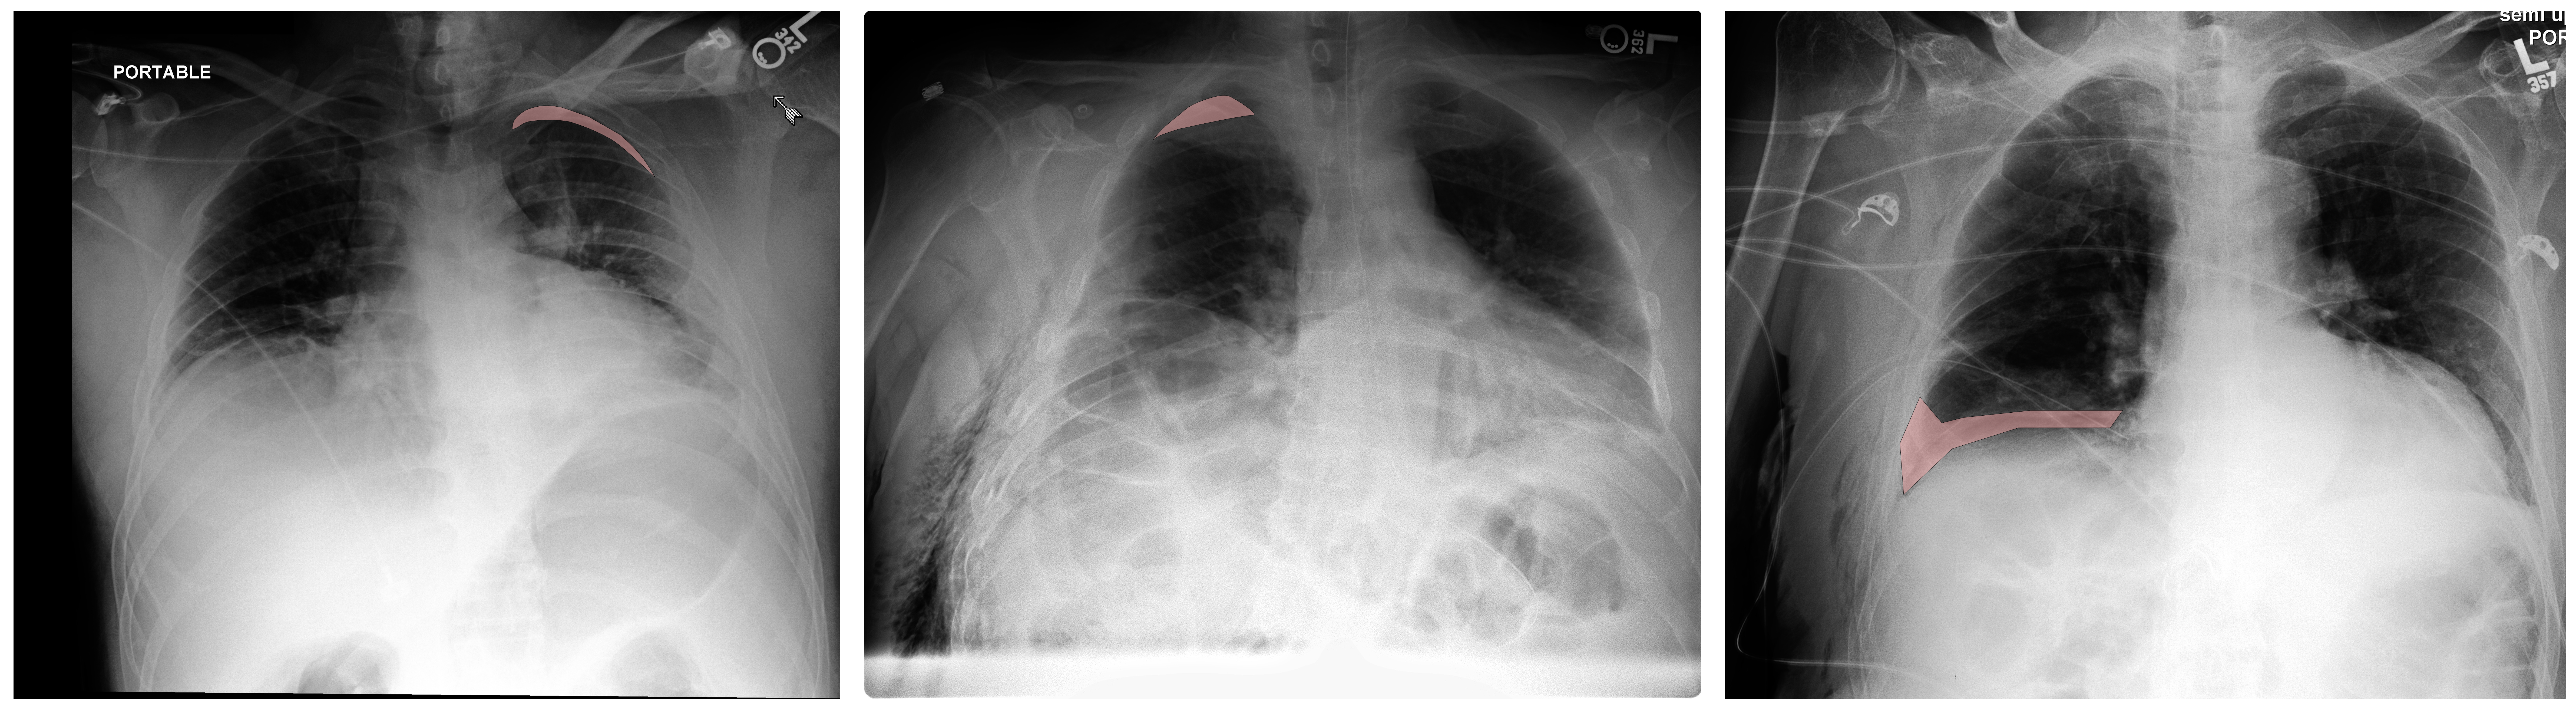
\includegraphics[width=0.75\textwidth]{figures/chest_pa_comparison.png}
  \caption{Chest X-ray Comparison by Hemoglobin Levels. Left: High (13.3 g/dL), Center: Median (10.77 g/dL), Right: Low (7.15 g/dL).}
  \label{fig:chest_comparison}
\end{figure}

하위 백분위수 환자(7.15 g/dL)는 multiple rib fractures로 인한 Hemo-pneumothorax가 확인되었으며, 직접적인 외상으로 인한 출혈이 헤모글로빈 저하를 유발하였다. 반면 상위 백분위수 환자(13.3 g/dL)는 cardiomegaly와 함께 diuretics 사용으로 인한 hemoconcentration이 관찰되었다. 중위값 환자(10.77 g/dL)는 임상적으로 경도 빈혈에 해당하나, 외상성 기흉 환자군 전반에서 출혈에 따른 헤모글로빈 저하가 흔함을 시사한다. 이는 헤모글로빈이 외상성 기흉의 중증도와 직결되는 출혈량 및 손상 범위를 대변하는 생리학적으로 타당한 지표임을 뒷받침한다. 단, 영상 분석은 레벨에 대해 각각 샘플 하나씩만을 분석한 것으로, 일반화를 하기에는 한계가 존재한다.

\section{논의}
본 과제에서는 원 논문의 주요 결과를 완전히 재현하는 데 한계가 있었다. 베이스라인 AUROC는 0.910으로 원 논문(0.979)보다 약 0.07 낮았으며, Recall은 0.442로 원 논문(0.730)보다 약 0.29 낮았다.

\subsection{재현 실패 요인 분석}
가장 근본적인 요인은 코호트 구성의 차이이다. 원 논문에서는 실험군 174명, 대조군 3,697명을 추출하였으나, 본 연구에서는 실험군 119명(약 32\% 감소), 대조군 544명(약 85\% 감소)만을 최종 분석에 포함할 수 있었다. 이는 중증 기흉 판별 기준의 상이함에서 기인한다. 원 논문은 흉부 X선 영상에서 직접 측정한 크기를 기준으로 중증도를 판별하였으나, 본 연구에서는 영상의학 보고서에 대한 텍스트 마이닝에 의존하였다. 또한, 원 논문에서는 결측치 처리에 사용된 구체적 알고리즘을 명시하지 않아 동일한 전처리 결과를 보장할 수 없었으며, 기존 연구의 논문 제출 시점(2019년)과 현재 사용한 MIMIC-IV 버전 간의 차이도 존재할 수 있다.

\subsection{과제의 한계점}
본 과제의 최종 실험군이 119명에 불과하여 모델의 통계적 안정성과 일반화 성능에 제약이 있었다. 5-Fold 교차 검증 결과의 표준편차가 상대적으로 높게 나타난 것(AUROC $\pm$ 0.040, Recall $\pm$ 0.100)은 소규모 데이터셋의 한계를 반영한다. 또한, 기존 연구에서 수행한 eICU 데이터셋을 활용한 외부 검증을 시간 및 자원의 제약으로 수행하지 못하여 제안 모델의 일반화 가능성을 객관적으로 평가할 수 없었다.

\subsection{임상적 함의}
제안 모델은 Recall 0.700을 달성하여 베이스라인(0.442) 대비 약 58\% 향상을 보였으나, 임상 현장 적용을 위해서는 추가적인 개선이 필요하다. 향후 연구에서는 다기관 데이터 통합을 통한 코호트 확대, 외부 데이터셋을 활용한 검증, 그리고 데이터 추출 쿼리 및 전처리 코드의 공개를 통한 재현성 향상이 필요하다.

\section{결론}
본 과제는 외상성 중증 기흉 예측을 위한 XGBoost 기반 머신러닝 모델의 재현 연구를 수행하였다. 기존 연구의 결과를 완전히 재현하는 데는 한계가 있었으나, 민감도 최적화를 통해 Recall을 0.442에서 0.700으로 향상시킨 모델을 제안하였다. 향후 연구에서는 외부 검증 및 코호트 확대를 통해 모델 일반화 성능 향상이 필요하다. 전체 소스 코드는 GitHub\footnote{\url{https://github.com/ga111o/mimic-pneumothorax-progression-analysis}}에서 확인할 수 있다.

\bibliographystyle{plain}
\bibliography{references}

\end{document}
